\section{Problem 4}
\label{part4}
\begin{verbatim}
4.  Repeat A3, Q1.  Compare the resulting text from February to 
the text you have now.  Do all 1000 URIs still return a ``200 OK'' 
as their final response (i.e., at the end of possible redirects)?

Create two graphs similar to that described in Q3, except this 
time the y-axis corresponds to difference in bytes (and not difference
in TimeMap magnitudes).  For the first graph, use the difference
in the raw (unprocessed) results.  For the second graph, use the 
difference in the processed (as per A3, Q1) results.

Of the URIs that still terminate in a ``200 OK'' response, pick the
top 3 most changed (processed) pairs of pages and use the Unix
``diff'' command to explore the differences in the version pairs.
\end{verbatim}
\subsection{Solution}
\begin{enumerate}

\item In this question I need to compare the resulting text from my 3rd Assignment and present resulting text.
\item In order to do this I have taken code from 3rd Assignment and executed it again and the code for this can be seen in the following listing\ref{lst:q4-1}.
\item This gives me a new set of raw and processed data files with complete updated text. Now I need to find the difference in the file sizes in bytes for each URI.
\item In order to subtract the old file sizes from the new file sizes I wrote a code for it which can be seen in the listing\ref{lst:q4-2}. 
\item This was a tough task because I need to do it for new raw and processed data and old raw and processed data which is very confusing as the data files are pretty similar.
\item I also checked for the status codes of all the URI's using the code in listing\ref{lst:q4-3}. I have found out that there are 891 URI's which give a status code of ``200''.
\item The list of other status codes can be seen in the table below.
\item I have then plotted a line graph using R which shows the differences in bytes for the files in old and new data. This code for this can be found in the listing\ref{lst:q4-4}.
\item Line graph showing the differences for the files sizes in bytes for raw data can be found in the fig\ref{Samplet41}.
\item Line graph showing the differences for the files sizes in bytes for processed data can be found in the fig\ref{Samplet42}.
\item Then my last task is to take a list of all URI's which return status code as ``200'' and from that list I need to pick top 3 most changed data files. This is done only for processed data files.
\item The top 3 URI's whose resulting text are mostly changed are ``http://www.gaynycdad.com/2016/02/giveaway-25-walmartsams-club-gift-card.html',``http://peanutbutterandwhine.com/februarys-50-your-way-giveaway-single-blog/'' and ``http://newsbunch.com/tech-news/track-cell-service-along-your-subway-route-with-this-new-app/''.
\item The changes for these particular URI's are compared using ``vim -d newdatafile olddatafile''.
\item When the above code in executed in putty it gives me the changes that occured in their text which are shown below.
\item The changes in the text files for 1st top most changed URI can be seen in the fig\ref{Samplet43}.
\item The changes in the text files for 2nd top most changed URI can be seen in the fig\ref{Samplet44}.
\item The changes in the text files for 3rd top most changed URI can be seen in the fig\ref{Samplet45}.

\end{enumerate}
\newpage
\begin{table}
\caption{Status code and their count}
\label{q4Table1}
\begin{center}
\hspace{-2cm}
\begin{tabular}{|c|c|}
\hline
 \textbf{Status codes} & \textbf{count}\\ \hline
  417  &	1 \\ \hline
 423 &   1 \\ \hline
 200 &	891  \\ \hline
 403 &  11	  \\ \hline
404 & 32\\ \hline
503 & 48\\ \hline
500 & 1\\ \hline
410 & 3\\ \hline
\end{tabular}
\end{center}
\end{table}
\newpage



\subsection{Code Listing }
\subsubsection{Code Listing 1}
\lstinputlisting[language=Python,breaklines = true,frame=single,caption={Python Code for getting raw and processed files for each URI}, label=lst:q4-1,captionpos=b,numbers=left,showspaces=false,showstringspaces=false,basicstyle=\footnotesize]{raw_and_processed_data.py}
\newpage

\subsubsection{Code Listing 2}

\lstinputlisting[language=python,breaklines = true,frame=single,caption={Python Code subtracting the new byte count and old byte count for raw and processed data files for 1000 URI's }, label=lst:q4-2,captionpos=b,numbers=left,showspaces=false,showstringspaces=false,basicstyle=\footnotesize]{subtraction.py}
\newpage

\subsubsection{Code Listing 3}

\lstinputlisting[language=python,breaklines = true,frame=single,caption={Python Code for checking the status codes of all the URI's}, label=lst:q4-3,captionpos=b,numbers=left,showspaces=false,showstringspaces=false,basicstyle=\footnotesize]{checkstatus.py}
\newpage

\subsubsection{Code Listing 4}

\lstinputlisting[language=R,breaklines = true,frame=single,caption={R code to plot a line graph to show the differences in bytes for old and new data}, label=lst:q4-4,captionpos=b,numbers=left,showspaces=false,showstringspaces=false,basicstyle=\footnotesize]{R_code2.R}

\subsection{Outputs}
\subsubsection{Output 1}
\begin{figure}[ht]    
    \begin{center}
        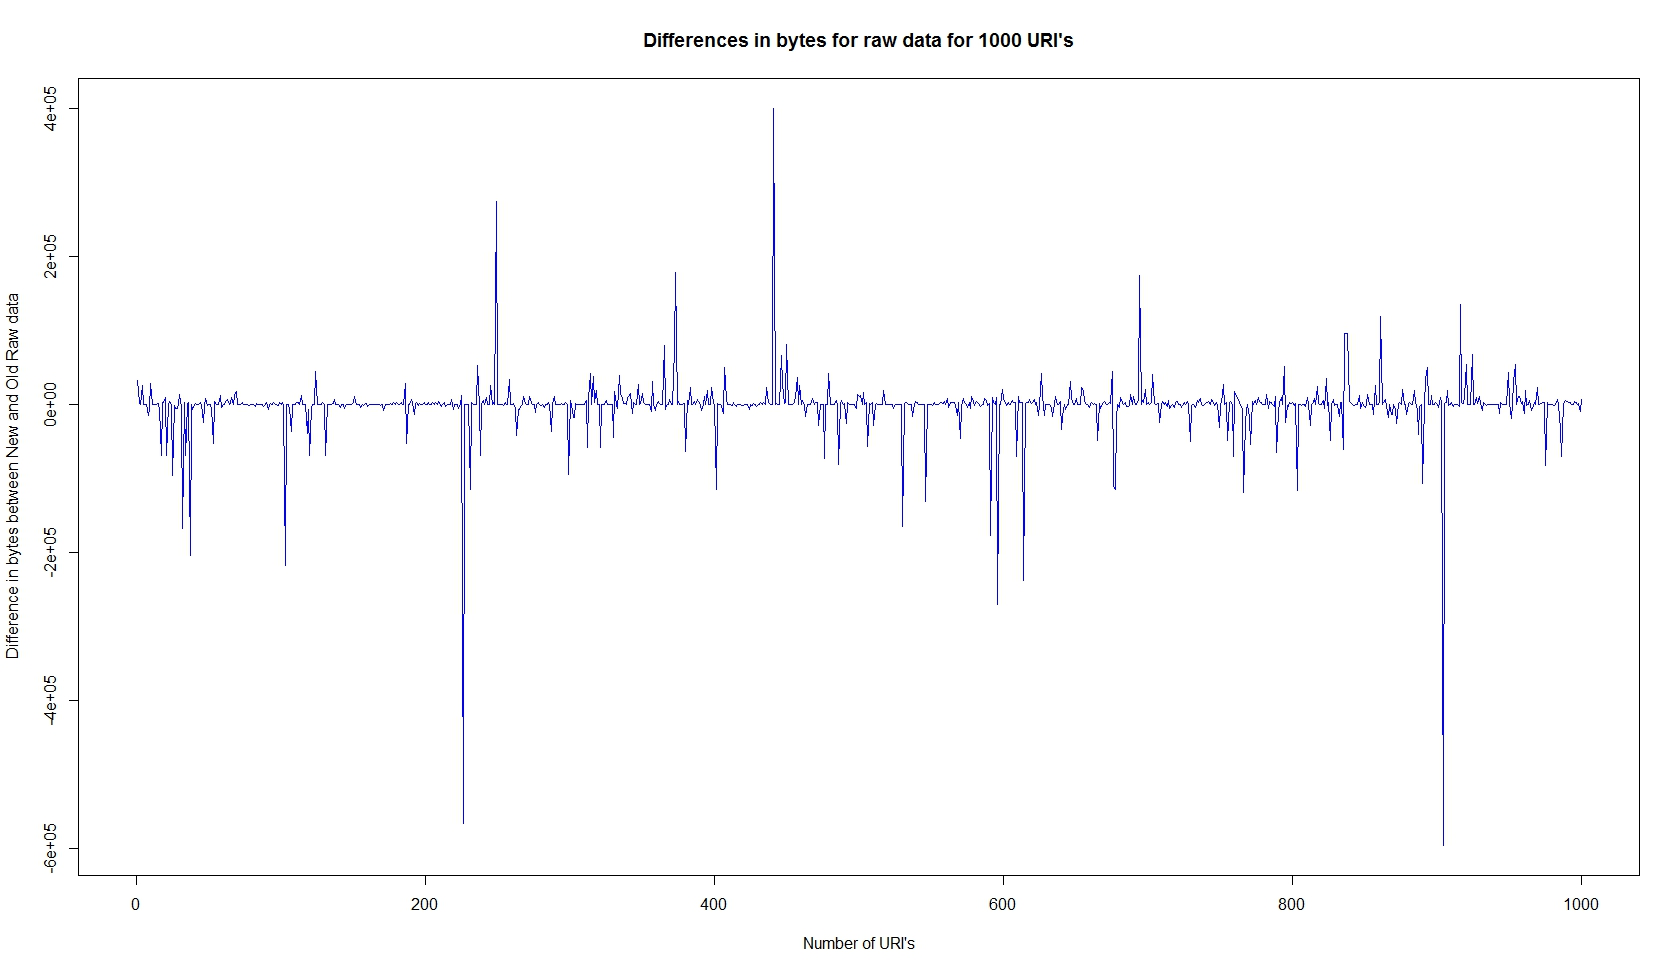
\includegraphics[scale=0.3]{raw_graph.jpeg}
        \caption{Line graph showing differences in bytes for raw data for 1000 URI's}
        \label{Samplet41}
    \end{center}
\end{figure}
\newpage

\subsubsection{Output 2}
\begin{figure}[ht]    
    \begin{center}
        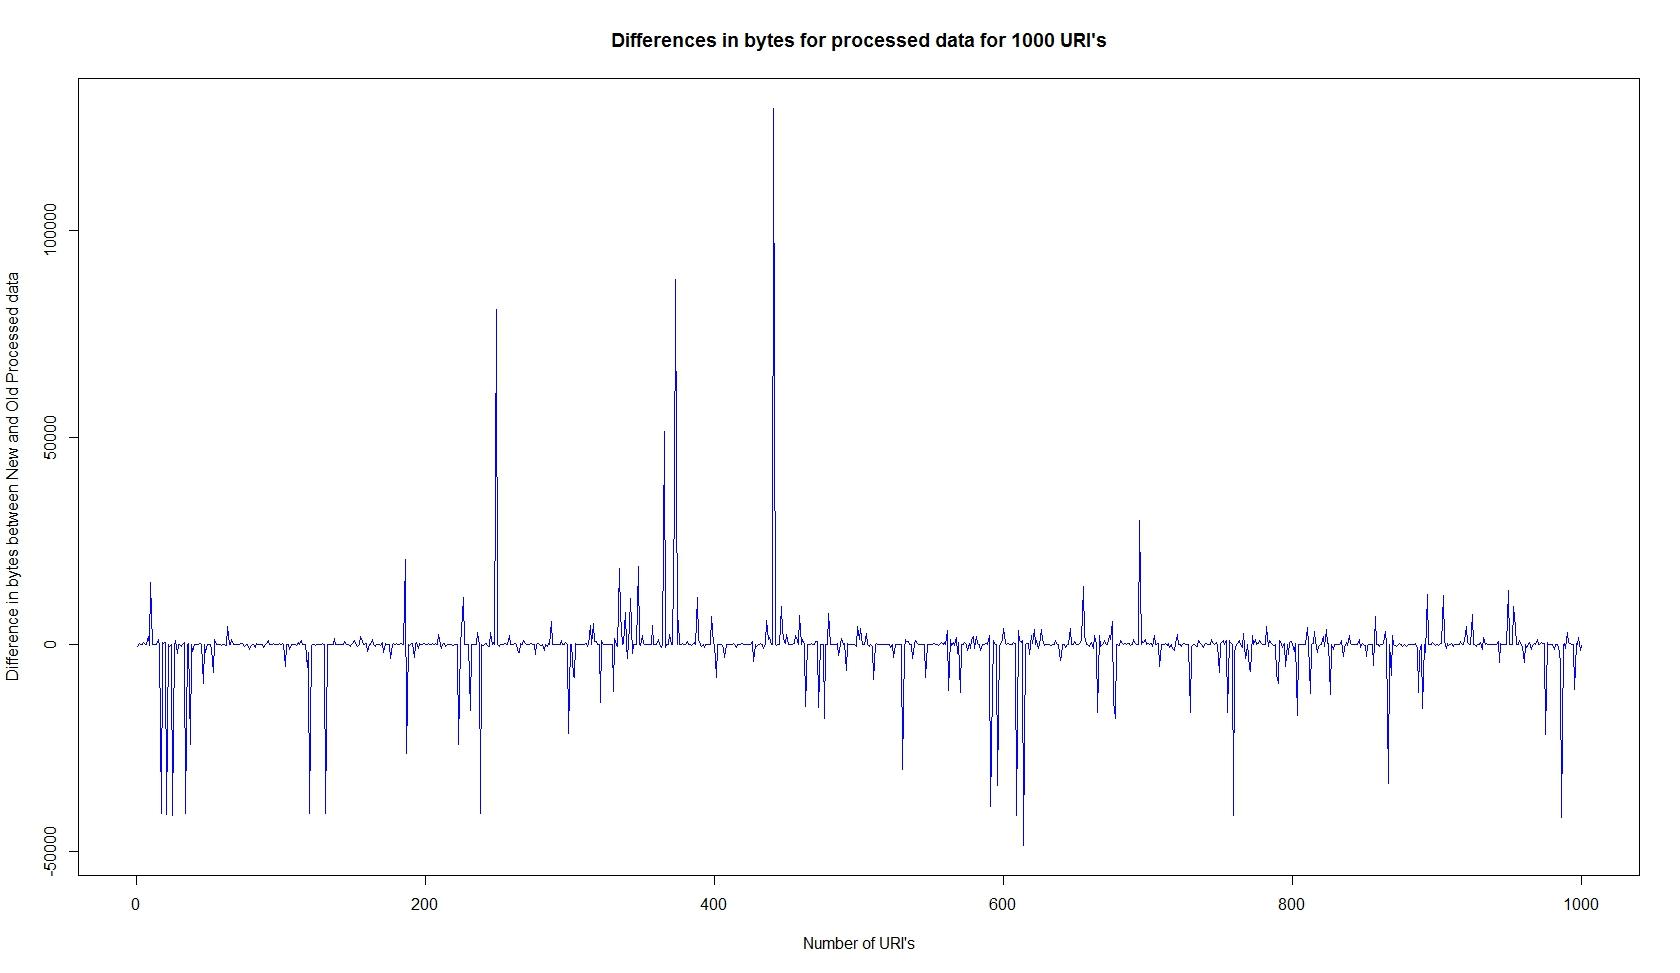
\includegraphics[scale=0.3]{processed_graph.jpeg}
        \caption{Line graph showing differences in bytes for processed data for 1000 URI's }
        \label{Samplet42}
    \end{center}
\end{figure}
\newpage


\subsubsection{Output 3}
\begin{figure}[ht]    
    \begin{center}
        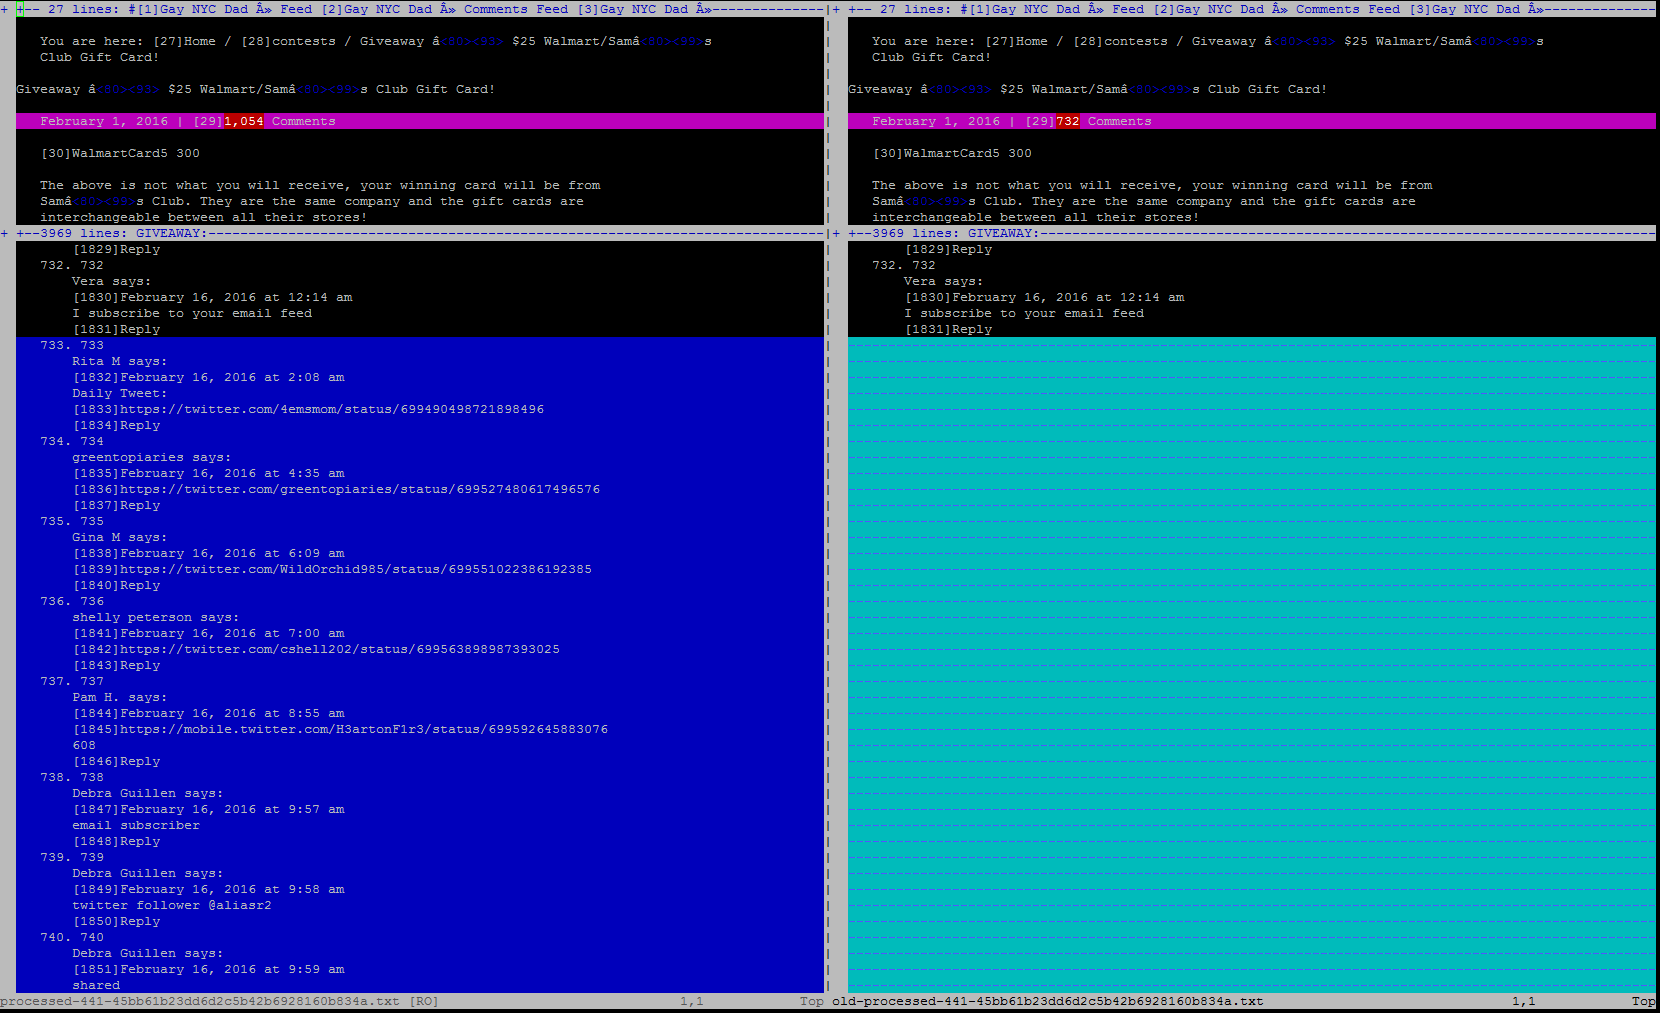
\includegraphics[scale=0.4]{output441.png}
        \caption{differences in old and new data plotted by vim -d for 1st top most changed URI }
        \label{Samplet43}
    \end{center}
\end{figure}
\newpage


\subsubsection{Output 4}
\begin{figure}[ht]    
    \begin{center}
        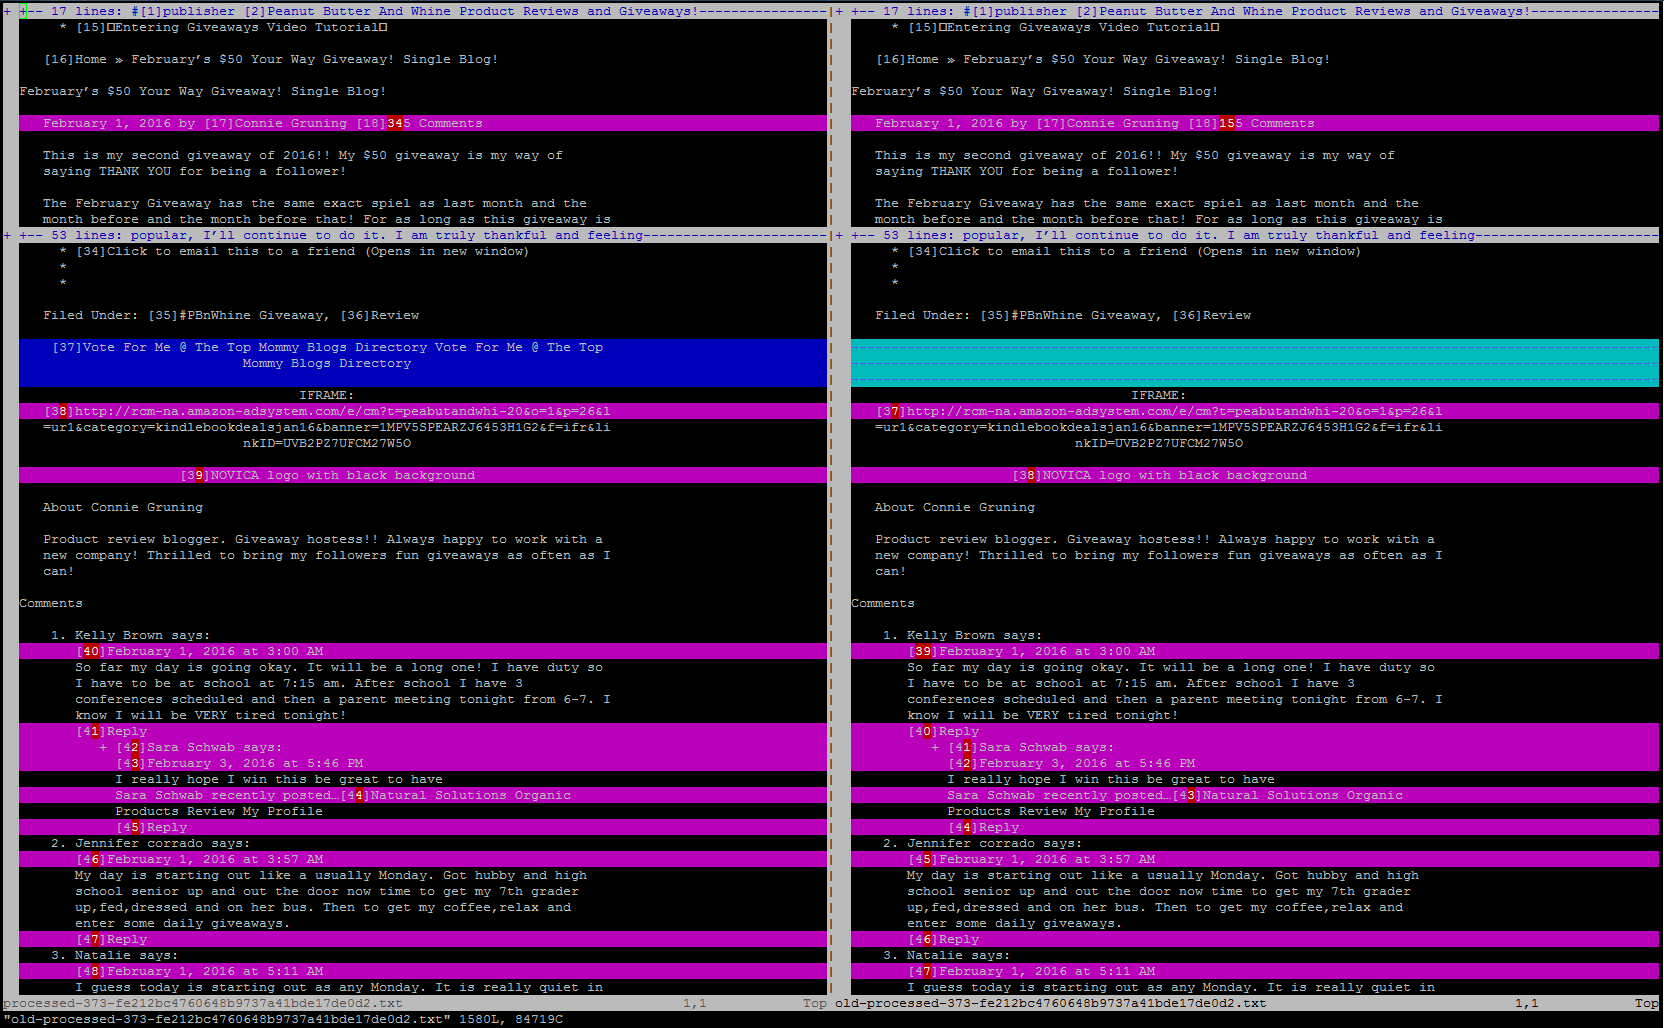
\includegraphics[scale=0.4]{output373.png}
        \caption{differences in old and new data plotted by vim -d for 2nd top most changed URI }
        \label{Samplet44}
    \end{center}
\end{figure}
\newpage


\subsubsection{Output 5}
\begin{figure}[ht]    
    \begin{center}
        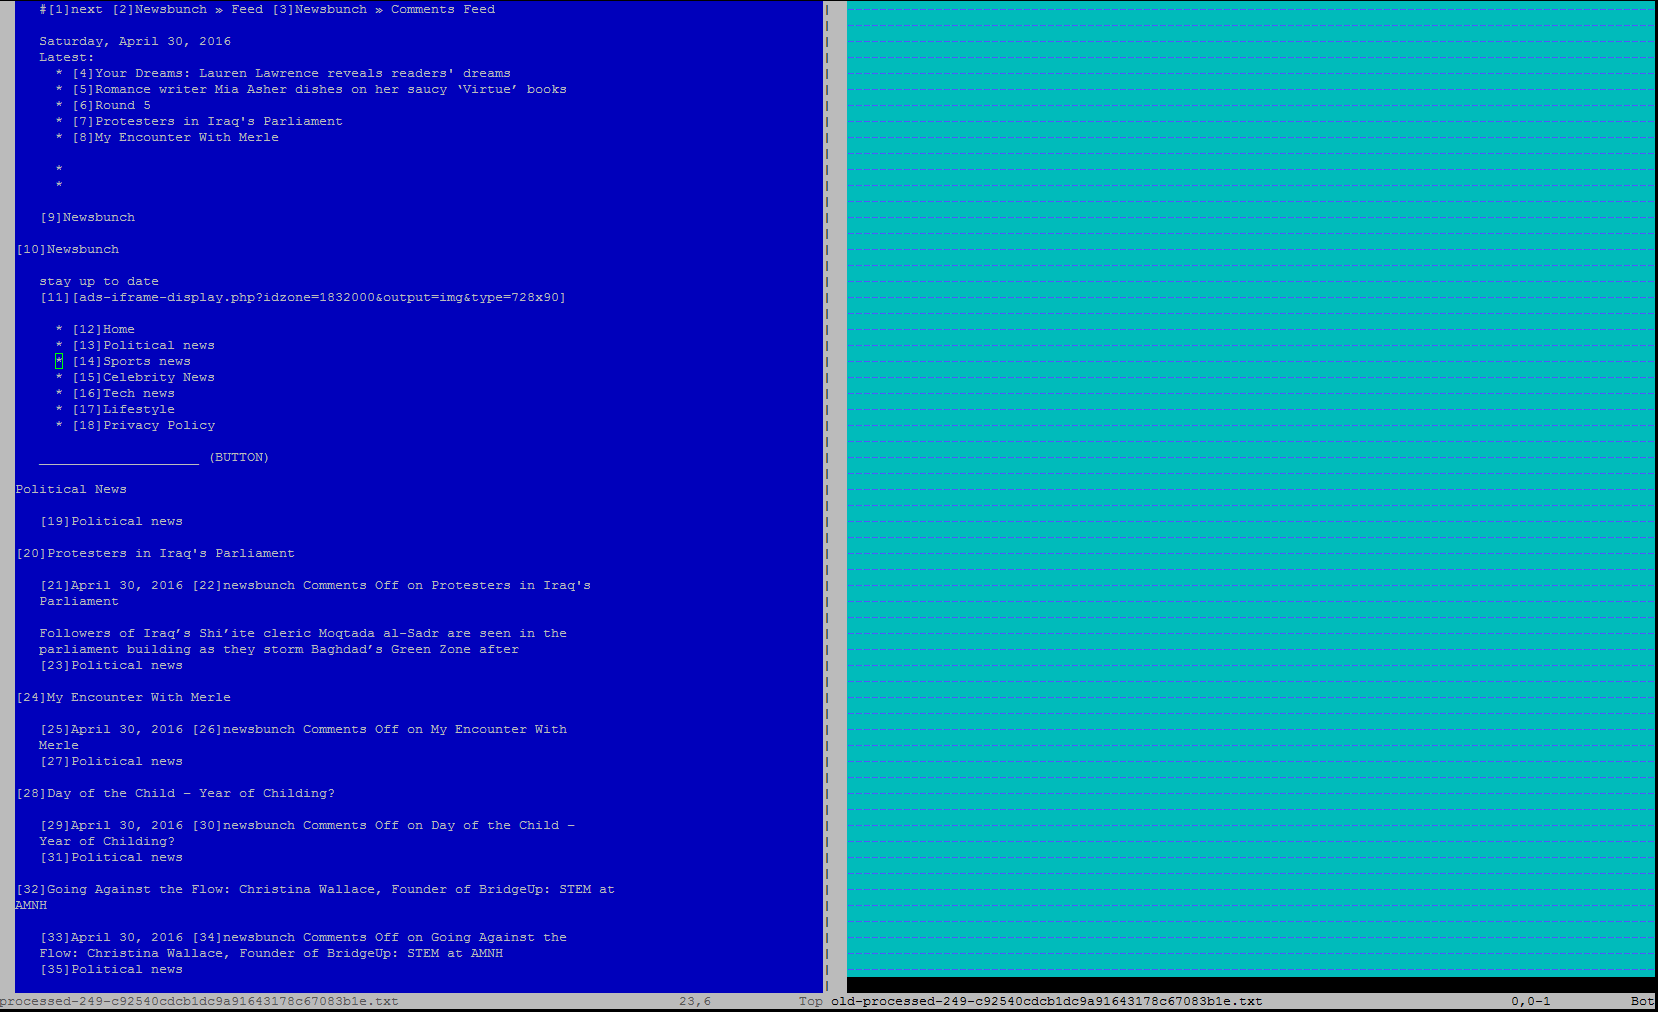
\includegraphics[scale=0.4]{output249.png}
        \caption{differences in old and new data plotted by vim -d for 3rd top most changed URI}
        \label{Samplet45}
    \end{center}
\end{figure}
\newpage



